\chapter{مفاهیم اولیه}

در این فصل به معرفی مقدمات و مفاهیم مورد نیاز در این پایان‌نامه می‌پردازیم.

\section{مقدمه}

در این فصل ابتدا به تاریخچه و تحولات هوش مصنوعی می‌پردازیم. سپس دسته‌بندی روش‌های یادگیری ماشین، الگوریتم‌های پایه، شبکه‌های عصبی بازگشتی و ساختار LSTM بررسی خواهد شد.



\subsection{آغاز هوش مصنوعی و هدف اصلی}

هوش مصنوعی به عنوان شاخه‌ای از علوم کامپیوتر، در دهه ۱۹۵۰ با هدف ساخت سیستم‌ها و ماشین‌هایی که توانایی تقلید از هوش انسانی را دارند، آغاز شد. نخستین بار، مکارتی در سال ۱۹۵۶ این اصطلاح را به کار گرفت \cite{mccarthy1956proposal} و هوش مصنوعی به عنوان علمی که در آن به مطالعه الگوریتم‌هایی برای تقلید رفتار انسانی می‌پردازد، شناخته شد. اهداف اولیه هوش مصنوعی شامل توانایی درک زبان، یادگیری، حل مسئله و تولید موجودات هوشمند بود. در این دوران پروژه‌های تحقیقاتی زیادی به امید دستیابی به هوش مصنوعی عمومی \footnote{\lr{AGI, Artificial General Intelligence}}
شروع به کار کردند \cite{crevier1993ai,nilsson2010quest}.

\subsection{دورهٔ طلایی و پیشرفت‌های اولیه}

در دههٔ ۵۰ و ۶۰ میلادی، هوش مصنوعی\footnote{\lr{Artificial Intelligence (AI)}} به عنوان یکی از پرچمداران پژوهش‌های نوین شناخته می‌شد. الگوریتم‌های اولیه با تکیه بر روش‌های منطقی و ریاضیاتی برای حل مسئله و بازی‌های ساده توسعه یافتند؛ مانند انواع الگوریتم‌های جستجوی درختی\footnote{\lr{Tree Search Algorithms}} که در این دوره به وجود آمدند و زمینه‌ساز اولین دستاوردهای هوش مصنوعی در بازی‌های تخته‌ای\footnote{\lr{Board Games}} همچون شطرنج\footnote{\lr{Chess}} شدند \cite{newell1959report}. 

در این دوران، پیشرفت‌های بیشتری در پردازش زبان طبیعی\footnote{\lr{Natural Language Processing (NLP)}} و سیستم‌های خبره\footnote{\lr{Expert Systems}} نیز صورت گرفت که این امید را در دانشمندان و محققان تقویت کرد که دستیابی به هوش مصنوعی عمومی\footnote{\lr{Artificial General Intelligence (AGI)}} به‌زودی ممکن خواهد بود \cite{feigenbaum1983handbook}.


\subsection{انتظارات بیش از حد و ظهور عصر تاریک}

با وجود پیشرفت‌های هوش مصنوعی، محدودیت‌های تکنولوژی (مثل عدم وجود  پردازنده های گرافیکی  \footnote{\lr{GPU}} پرقدرت در آن زمان) و همچنین کمبود داده‌های کافی برای آموزش مدل‌های پیچیده‌تر، باعث شد که بسیاری از پروژه‌های تحقیقاتی نتوانند به نتایج پیش‌بینی‌شده قابل قبول دست یابند. در نتیجه، هوش مصنوعی در دههٔ ۷۰ به مرحله‌ای از رکود وارد شد که به آن عصر تاریک هوش مصنوعی یا زمستان هوش مصنوعی \footnote{\lr{AI Winter}} می‌گویند \cite{lighthill1973artificial,crevier1993ai}. در این دوران، بسیاری از پروژه‌ها تعطیل و سرمایه‌گذاری‌ها قطع شدند و دولت‌ها و سازمان‌های سرمایه‌گذار به دلیل عدم دستیابی به نتایج مطلوب از ادامه سرمایه‌گذاری منصرف شدند.


\subsection{عوامل اصلی عصر تاریک هوش مصنوعی}

\begin{itemize}
	\item \textbf{محدودیت‌های سخت‌افزاری:}  
	در آن زمان، سیستم‌های اولیه هوش مصنوعی به محاسبات سنگینی نیاز داشتند که با توان پردازشی محدود آن دوره همخوانی نداشت \cite{nilsson2010quest}.
	
	\item \textbf{کمبود داده‌ها:}  
	در آن زمان، دسترسی به داده‌های کافی برای آموزش مدل‌های پیچیده ممکن نبود و الگوریتم‌های موجود به داده‌های بیشتری نیاز داشتند تا بتوانند به‌درستی آموزش ببینند و عملکرد مطلوبی داشته باشند \cite{crevier1993ai}.
	
	\item \textbf{روش‌های محدود یادگیری:}  
	الگوریتم‌های اولیه به شدت به برنامه‌ریزی انسانی وابسته بودند و در بسیاری از موارد، مدل‌ها قادر به تعمیم به مسائل جدید نبودند و نمی‌توانستند تعمیم‌پذیری خیلی بالایی داشته باشند \cite{russell2016artificial}.
\end{itemize}

\subsection{پایان عصر تاریک و بازگشت هوش مصنوعی}

پس از چندین سال رکود و عدم سرمایه‌گذاری در حوزهٔ هوش مصنوعی، سرانجام در دههٔ ۱۹۸۰ و ۱۹۹۰ عصر تاریک هوش مصنوعی با تحولات تکنولوژی و از همه مهم‌تر ظهور سیستم‌های خبره به پایان رسید \cite{feigenbaum1983handbook}. سیستم‌های خبره به عنوان یکی از اولین تلاش‌های موفق برای کاربردهای صنعتی در هوش مصنوعی به‌وجود آمدند. بر خلاف الگوریتم‌های اولیه، این سیستم‌ها از پایگاه بزرگ قواعد و قوانین \footnote{\lr{\lr{Rule Based Systems}}} استفاده می‌کردند. در سیستم‌های خبره، به جای تلاش برای شبیه‌سازی کلی هوش مصنوعی، بر حل مسائل تخصصی برای صنایع و سازمان‌ها تمرکز می‌شد. برای مثال، سیستم‌های خبره در پزشکی برای تشخیص بیماری‌ها و پیشنهاد درمان، در صنعت برای مدیریت و پیش‌بینی خرابی ماشین‌آلات، و در امور مالی برای تحلیل و ارزیابی ریسک کاربرد داشتند \cite{mccorduck2004machines}.

هرچند این سیستم‌ها نمی‌توانستند درک عمیق و هوشمندی عمومی را ایجاد کنند، اما برای رفع نیازهای پیچیده مناسب بودند. همزمان با موفقیت این سیستم‌ها، بهبودهای زیادی در سخت‌افزارها و کاهش هزینه‌های پردازش به وجود آمد. در دهه‌های ۱۹۸۰ و ۱۹۹۰، کامپیوترها به تدریج قوی‌تر و مقرون به صرفه‌تر شدند و امکان پردازش داده‌های بیشتر و اجرای الگوریتم‌های پیچیده‌تر فراهم شد. این افزایش توان محاسباتی، نیاز به پردازش داده‌های بزرگ و پیچیده را برآورده کرد و در نتیجه دسترسی به داده‌ها و انجام محاسبات سنگین برای توسعه الگوریتم‌های جدید تسهیل شد. از سوی دیگر، پیشرفت‌های انجام‌شده در ذخیره‌سازی داده و رشد اینترنت باعث دسترسی گسترده‌تر به داده‌ها و منابع اطلاعاتی گردید \cite{nilsson2010quest}.

به این ترتیب، مجموعه‌ای از عوامل، شامل ظهور سیستم‌های خبره، افزایش قدرت پردازش و دسترسی به داده‌های بیشتر، منجر به بازگشت هوش مصنوعی شد. این دوره نه تنها پایان عصر تاریک هوش مصنوعی بود، بلکه راه را برای الگوریتم‌های یادگیری ماشین و توسعهٔ شبکه‌های عصبی هموار کرد \cite{russell2016artificial}.


\section{انواع مدل یادگیری ماشین و شبکه‌های عصبی}\label{sec:ml-types}
یادگیری ماشین و شبکه‌های عصبی به عنوان دو زیرشاخه مهم از هوش مصنوعی، در سال‌های اخیر به‌طور گسترده‌ای مورد توجه پژوهشگران و صنعت قرار گرفته‌اند. این مدل‌ها با هدف یادگیری الگوها و روابط موجود در داده‌ها توسعه یافته‌اند و امروزه در حوزه‌های مختلفی از جمله بینایی ماشین، پردازش زبان طبیعی، پیش‌بینی سری‌های زمانی و داده‌کاوی مورد استفاده قرار می‌گیرند \cite{bishop2006pattern,mitchell1997machine,murphy2012machine}.

\subsection{یادگیری ماشین: مروری کلی}
یادگیری ماشین \footnote{\lr{Machine Learning}} شاخه‌ای از هوش مصنوعی است که به مدل‌های محاسباتی این امکان را می‌دهد الگوها را از داده‌ها به شکل خودکار یاد بگیرند و بتوانند تصمیم‌گیری کنند
\cite{goodfellow2016deep,mitchell1997machine}.
در واقع، هدف یادگیری ماشین این است که مدل‌ها بتوانند از داده‌ها الگوها و روابط پنهان را استخراج کنند و به نتایج و تصمیم‌های قابل اعتماد دست یابند.

\subsection{تقسیم‌بندی‌های اصلی در یادگیری ماشین}
به طور کلی، یادگیری ماشین به سه دستهٔ اصلی تقسیم می‌شود:
\begin{itemize}
 	\item یادگیری با نظارت\footnote{\lr{Supervised Learning}}
	\item یادگیری بدون نظارت\footnote{\lr{Unsupervised Learning}}
	\item یادگیری تقویتی\footnote{\lr{Reinforcement Learning}}	
\end{itemize}
این طبقه‌بندی در بسیاری از کتاب‌ها و مراجع مهم یادگیری ماشین مطرح شده است
\cite{bishop2006pattern,murphy2012machine}.

\subsection{یادگیری نظارت‌شده}
یادگیری نظارت‌شده یکی از رایج‌ترین روش‌ها در یادگیری ماشین شناخته می‌شود که در آن از مجموعه داده‌های برچسب‌گذاری‌شده برای آموزش مدل استفاده می‌کنیم \cite{james2013introduction}. هدف این الگوریتم تشخیص الگوها در میان داده‌های ورودی است تا بتواند روی داده‌های جدید پیش‌بینی یا طبقه‌بندی انجام دهد. این نوع شامل دو دسته الگوریتم رگرسیون \footnote{\lr{Regression}} و کلاس بندی\footnote{\lr{Classification}} می‌شود.



\subsection{طبقه‌بندی}
طبقه‌بندی یکی از مهم‌ترین و اصلی‌ترین وظایف در یادگیری نظارت‌شده است که هدف آن تخصیص هر داده به یک لیبل\footnote{\lr{Label}} مشخص است
\cite{bishop2006pattern}.
در این روش، مدل با داده‌های برچسب‌دار آموزش می‌بیند و یاد می‌گیرد که داده‌های جدید را بر اساس الگوها و ویژگی‌هایی که در داده‌های آموزشی دیده است، به دسته مناسب اختصاص دهد. از کاربردهای طبقه‌بندی می‌توان به تشخیص هرزنامه،
 \footnote{\lr{Spam Detection}} تشخیص بیماری و تشخیص چهره اشاره کرد.\cite{murphy2012machine}.

\subsection{رگرسیون}
رگرسیون \footnote{\lr{regression}} یکی از مهم‌ترین وظایف یادگیری ماشین است و هدف آن پیش‌بینی مقادیر پیوسته است
\cite{montgomery2021introduction}. بر خلاف طبقه‌بندی که خروجی آن یک دسته‌بندی مجزا است، در رگرسیون خروجی یک مقدار پیوسته خواهد بود و مدل می‌آموزد روابط بین متغیرهای مستقل و متغیر هدف را شناسایی کند. از کاربردهای رگرسیون می‌توان به پیش‌بینی قیمت مسکن یا پیش‌بینی آب‌وهوا اشاره کرد.

\subsection{یادگیری تقویتی}
یادگیری تقویتی، \footnote{\lr{reinforcement learning}} نوعی یادگیری بر پایهٔ پاداش و تنبیه است که در آن مدل با محیط تعامل می‌کند و بر اساس پاداش یا تنبیه یاد می‌گیرد
\cite{sutton2018reinforcement}.
برخلاف یادگیری نظارت‌شده و بدون نظارت، یادگیری تقویتی به مدل این امکان را می‌دهد تا از طریق آزمون و خطا بهترین راهکارها را برای انجام یک عمل یاد بگیرد. در این روش، مدل به جای برچسب، از یک تابع پاداش استفاده می‌کند که مشخص می‌کند چه اقداماتی باعث نتیجه بهینه می‌شود. از کاربردهای یادگیری تقویتی می‌توان به بازی‌ها \footnote{\lr{Games}}، کنترل رباتیک \footnote{\lr{Robotic Control}} و سیستم‌های توصیه‌گر \footnote{\lr{Recommender Systems}} اشاره کرد.



\subsection{معرفی چند مدل از الگوریتم یادگیری کلاسیک}

الگوریتم‌های یادگیری کلاسیک، پایه و اساس بسیاری از پیشرفت‌های اولیه در یادگیری ماشین را شکل داده‌اند. این الگوریتم‌ها با وجود سادگی نسبی، در بسیاری از کاربردها همچنان عملکرد قابل قبولی از خود نشان می‌دهند و در بسیاری از سامانه‌های عملیاتی مورد استفاده قرار می‌گیرند.

الگوریتم‌هایی مانند نزدیک‌ترین همسایه، ماشین بردار پشتیبان، بیز ساده و درخت تصمیم از جمله مشهورترین روش‌های کلاسیک یادگیری هستند که هر یک بر اساس اصول ریاضی و آماری متفاوتی طراحی شده‌اند. این مدل‌ها معمولاً برای مسائل طبقه‌بندی یا رگرسیون به‌کار می‌روند و از مزایایی چون پیاده‌سازی آسان، قابلیت تفسیر بالا و نیاز کمتر به تنظیمات پیچیده برخوردارند.

در این بخش، به معرفی اجمالی چند مورد از این الگوریتم‌ها پرداخته می‌شود تا زمینهٔ درک عمیق‌تر روش‌های نوین‌تر یادگیری، مانند شبکه‌های عصبی و مدل‌های عمیق، فراهم گردد.

\subsection{نزدیک‌ترین همسایه }

الگوریتم نزدیک‌ترین همسایه \footnote{\lr{k-Nearest Neighbors}} یکی از روش‌های ساده و درعین‌حال کارآمد در یادگیری نظارت‌شده است که هم در دسته‌بندی و هم در رگرسیون کاربرد دارد
\cite{cover1967nearest,duda1973pattern,mitchell1997machine}.
این الگوریتم برای پیش‌بینی دسته‌بندی یک نمونهٔ جدید، به $k$ نزدیک‌ترین داده‌ها در فضای ویژگی نگاه می‌کند و بر اساس اکثریت نزدیکی همسایه‌ها، آن را به یک دسته اختصاص می‌دهد. 

\subsubsection{مزایا:}
\begin{itemize}
	\item \textbf{سادگی و قابل فهم بودن:}  
	این الگوریتم به سادگی با اندازه‌گیری فاصله بین نقاط داده کار می‌کند و بدون نیاز به آموزش مدل پیچیده قابل استفاده است
	\cite{cover1967nearest}.
	\item \textbf{عملکرد خوب در داده‌های با تعداد ویژگی کم:}  
	در مسائلی که تعداد ویژگی‌ها کم است، این الگوریتم اغلب به خوبی عمل می‌کند
	\cite{james2013introduction}.
\end{itemize}

\subsubsection{معایب:}
\begin{itemize}
	\item \textbf{حساسیت به داده‌های پرت:}  
	نقاط پرت می‌توانند به‌طور قابل توجهی بر نتایج تأثیر بگذارند
	\cite{duda1973pattern}.
	\item \textbf{کندی در داده‌های بزرگ:}  
	این الگوریتم نیاز به محاسبه فاصله برای هر نقطهٔ جدید دارد و در داده‌های بزرگ بار محاسباتی بالایی خواهد داشت
	\cite{mitchell1997machine}.
	\item \textbf{عدم کارایی در داده‌های با ابعاد بالا:}  
	در داده‌هایی با تعداد ویژگی‌های زیاد، کارایی الگوریتم کاهش می‌یابد \cite{murphy2012machine}.
\end{itemize}



\subsection{ماشین بردار پشتیبان}
الگوریتم ماشین بردار پشتیبان \footnote{\lr{Support Vector Machine, SVM}} با یافتن یک ابرصفحهٔ بهینه، داده‌ها را به کلاس‌های مختلف تقسیم می‌کند
\cite{cortes1995support,vapnik1998statistical}.
این الگوریتم یک ابرصفحه به دست می‌آورد که هدف آن حداکثر کردن فاصله میان داده‌های دو کلاس است و به این ترتیب می‌تواند طبقه‌بندی دقیقی داشته باشد.

\subsubsection{مزایا:}
\begin{itemize}
	\item \textbf{توانایی مقابله با داده‌های پیچیده و ابعاد بالا:}
	\lr{SVM} می‌تواند به خوبی با داده‌های چندبعدی و پیچیده کار کند
	\cite{vapnik1998statistical}.
	\item \textbf{مقاومت در برابر بیش‌برازش \footnote{\lr{Overfitting}}:}
با استفاده از هسته‌ها \footnote{\lr{kernels}}، داده‌های غیرخطی نیز به فضای بالاتر برده می‌شوند و جداسازی بهتری انجام می‌شود\cite{cortes1995support}.
\end{itemize}

\subsubsection{معایب:}
\begin{itemize}
	\item \textbf{پیچیدگی محاسباتی:}
	آموزش ماشین بردار پشتیبان به دلیل نیاز به حل مسائل بهینه‌سازی، در حجم‌های بالای داده محاسباتی زمان‌بر است
	\cite{murphy2012machine}.
	\item \textbf{کارایی پایین در داده‌های پرت:}
	در صورتی که داده‌ها شامل نقاط پرت زیادی باشند، دقت مدل کاهش می‌یابد
	\cite{bishop2006pattern}.
\end{itemize}


\subsection{بیز ساده}
بیز ساده \footnote{Naive Bayes} مبتنی بر قضیه بیز \footnote{\lr{Bayes' theorem}}است و فرض می‌کند ویژگی‌ها به‌صورت شرطی مستقل از هم هستند\cite{domingos1997optimal,mitchell1997machine}.
این مدل برای اولین بار در حوزهٔ پردازش متن به کار رفت و هنوز هم در بسیاری از کاربردها مانند طبقه‌بندی ایمیل و تحلیل احساسات مورد استفاده قرار می‌گیرد\cite{mccallum1998comparison}. 
در بیز ساده بر اساس احتمالات محاسبه می‌شود که یک نمونهٔ جدید به کدام دسته تعلق دارد. این الگوریتم بر اساس قضیهٔ بیز، احتمال تعلق یک نمونه به هر دسته را به ازای هر ویژگی محاسبه کرده و در نهایت بالاترین احتمال را به‌عنوان جواب نهایی در نظر می‌گیرد\cite{bishop2006pattern}.

\subsubsection{مزایا:}
\begin{itemize}
	\item \textbf{سرعت بالا}: به دلیل محاسبات ساده و فرض استقلال ویژگی‌ها، بیز ساده بسیار سریع و کم‌حجم است
	\cite{mccallum1998comparison}.
	\item \textbf{کارایی در داده‌های کوچک}: حتی با داده‌های کم، این الگوریتم عملکرد نسبتاً خوبی دارد\cite{murphy2012machine}.
\end{itemize}

\subsubsection{معایب:}
\begin{itemize}
	\item \textbf{فرض استقلال ویژگی‌ها}: فرض استقلال ویژگی‌ها ممکن است در بسیاری از مسائل واقعی صادق نباشد و این می‌تواند دقت مدل را کاهش دهد
	\cite{domingos1997optimal}.
	\item \textbf{حساسیت به داده‌های نادرست}: در صورت وجود داده‌های نادرست یا پرت، مدل ممکن است دقت کمتری داشته باشد
	\cite{bishop2006pattern}.
\end{itemize}


\subsection{شبکه‌های عصبی بازگشتی و شبکه‌های حافظه بلندمدت کوتاه‌مدت}
شبکه‌های عصبی بازگشتی \footnote{\lr{RNN}} و مدل‌هایی با حافظهٔ بلندمدت-کوتاه‌مدت \footnote{\lr{LSTM}} با هدف پردازش داده‌های ترتیبی و وابسته به زمان توسعه یافتند
\cite{rumelhart1986learning,hochreiter1997long}.
این مدل‌ها به‌ویژه در تحلیل زبان طبیعی، پردازش صوت و پیش‌بینی سری‌های زمانی بسیار موفق عمل کرده‌اند؛ زیرا قادر به حفظ اطلاعات گذشته هستند و از این اطلاعات برای پیش‌بینی در لحظهٔ حال و آینده استفاده می‌کنند
\cite{gers1999learning}.

\subsection{شبکه‌های عصبی بازگشتی}
مدل‌های اولیهٔ شبکه‌های عصبی، مانند شبکه‌های چندلایه \footnote{\lr{MLP}}، قادر به پردازش داده‌های مستقل و ثابت بودند و نمی‌توانستند وابستگی‌های زمانی را یاد بگیرند\cite{bishop2006pattern}.
در بسیاری از مباحث دنیای واقعی مانند تحلیل متن، صدا و  داده‌ها به توالی خاصی وابسته هستند. به همین دلیل، شبکه‌های عصبی بازگشتی معرفی شدند تا بتوانند از اطلاعات پیشین در پردازش داده‌های بعدی استفاده کنند\cite{rumelhart1986learning}.



 \begin{figure}[h]
	\centering
	\begin{minipage}[b]{0.7\textwidth}
		\centering
		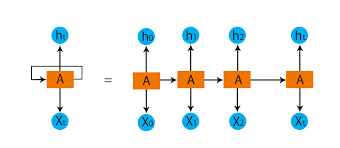
\includegraphics[width=\textwidth]{transformer_images/rnn_image.png}
		\caption{RNN}
		\label{fig:RNN}
	\end{minipage}
	\hfill
	
\end{figure}








\subsection{ساختار و عملکرد شبکه‌های عصبی بازگشتی}
شبکه‌های شبکه‌های عصبی بازگشتی دارای حلقهٔ بازگشتی هستند که به مدل این امکان را می‌دهد اطلاعات را در توالی نگه دارد و در هر گام زمانی، ورودی فعلی \( x_t \) و وضعیت قبلی \( h_{t-1} \) را به‌عنوان ورودی دریافت کند\cite{goodfellow2016deep}.
\begin{equation}
	h_t = \sigma \big( W \cdot x_t + U \cdot h_{t-1} + b \big)
\end{equation}

در اینجا:
\begin{itemize}
	\item \( h_t \) وضعیت مخفی یا حالت در گام زمانی \( t \) است.
	\item \( W \) وزن‌هایی است که به ورودی \( x_t \) اعمال می‌شود.
	\item \( U \) وزن‌های اعمال‌شده به وضعیت قبلی \( h_{t-1} \) است.
	\item \( b \) بایاس مدل است.
	\item \( \sigma \) تابع فعال‌سازی، معمولاً تانژانت هیپربولیک یا سیگموید.
\end{itemize}

با استفاده از این فرایند، مدل این توانایی را دارد که اطلاعات گذشته را در خود ذخیره کرده و در پردازش‌های بعدی از آن‌ها بهره ببرد.

\subsection{مزایا و معایب شبکه‌های عصبی بازگشتی}
در این قسمت به مزایا و معایب شبکه‌های شبکه‌های عصبی بازگشتی می‌پردازیم.

\subsubsection{مزایا:}
\begin{itemize}
	\item \textbf{حفظ وابستگی زمانی:}  
شبکه‌های عصبی بازگشتی قادر به پردازش توالی‌های طولانی است و می‌تواند اطلاعات را در طول توالی به خاطر بسپارد
	\cite{elman1990finding}.
	
	\item \textbf{کاربردهای گسترده در داده‌های ترتیبی:}  
	این مدل در تحلیل زبان طبیعی، پیش‌بینی سری‌های زمانی و پردازش صوت بسیار موفق عمل می‌کند
	\cite{gers1999learning}.
\end{itemize}

\subsubsection{معایب:}
\begin{itemize}
\item \textbf{مشکل ناپدید شدن و انفجار گرادیان \footnote{\lr{Vanishing and Exploding Gradient}}:}
در فرایند آموزش با روش پس‌انتشار، اگر توالی داده‌ها طولانی باشد، گرادیان‌ها ممکن است بسیار کوچک یا بزرگ شوند که منجر به ناپایداری در آموزش و کاهش دقت می‌شود
	\cite{hochreiter1998vanishing}.
	
	\item \textbf{محدودیت در پردازش توالی‌های بسیار بلند:}  
 شبکه‌های عصبی بازگشتی در حفظ اطلاعات طولانی‌مدت با مشکل مواجه است و برای پردازش وابستگی‌های طولانی، عملکرد ضعیفی دارد
	\cite{hochreiter1997long,goodfellow2016deep}.
\end{itemize}

\subsection{شبکه‌های حافظه بلندمدت-کوتاه‌مدت}

شبکه‌های حافظه بلندمدت-کوتاه‌مدت به عنوان یک راه‌حل برای یکی از بزرگ‌ترین مشکلات شبکه‌های عصبی بازگشتی معرفی شدند
\cite{hochreiter1997long}.
یکی از برجسته‌ترین مشکلات موجود در شبکه‌های عصبی بازگشتی، معضل ناپدید شدن گرادیان  بود که مانع یادگیری وابستگی‌های بلندمدت می‌شد
\cite{hochreiter1998vanishing,goodfellow2016deep}.
برای درک عمیق‌تر این مسأله، ابتدا به توضیح مشکل ناپدید شدن گرادیان و سپس راهکار شبکه‌های حافظه بلندمدت-کوتاه‌مدت می‌پردازیم.

\subsection{ناپدید شدن گرادیان در شبکه های بازگشتی}
شبکه‌های عصبی بازگشتی برای پردازش داده‌های ترتیبی از حلقه‌های بازگشتی بهره می‌برند. در فرایند آموزش شبکه‌های عصبی بازگشتی، از الگوریتم پس‌انتشار خطا از طریق زمان \footnote{\lr{Backpropagation Through Time}} استفاده می‌شود که گرادیان‌ها را جهت به‌روزرسانی وزن‌ها محاسبه می‌کند.\cite{rumelhart1986learning}.

با این حال، شبکه های عصبی بازگشتی در یادگیری وابستگی‌های بلندمدت معمولاً ناکام می‌مانند. علت اصلی این امر شامل موارد زیر است:

\begin{itemize}
	\item \textbf{ضریب‌های بازگشتی کوچک‌تر از ۱:}
	در فرایند محاسبهٔ گرادیان‌ها، اگر مقدار مشتقات یا ضرایب در هر مرحله کوچک‌تر از ۱ باشد، ضرب مکرر این ضرایب در طول توالی منجر به کوچک‌شدن گرادیان‌ها به سمت صفر می‌شود؛ پدیده‌ای که به ناپدید شدن گرادیان\footnote{\lr{vanishing gradient}} معروف است
	\cite{hochreiter1998vanishing}.
\end{itemize}

فرمول کلی گرادیان در زمان \( t \) به‌صورت زیر است:

\begin{equation}
	\frac{\partial L}{\partial W} = \prod_{k=1}^{t} \frac{\partial h_k}{\partial h_{k-1}} \cdot \frac{\partial h_t}{\partial L}
\end{equation}

در این فرمول، \( \frac{\partial h_k}{\partial h_{k-1}} \) ممکن است مقداری کوچک‌تر از ۱ باشد، و ضرب مکرر آن در طول توالی باعث کاهش شدید مقدار گرادیان می‌گردد.

\begin{itemize}
	\item \textbf{تأثیر مستقیم بر وزن‌ها:}
	زمانی که گرادیان‌ها به صفر نزدیک می‌شوند، وزن‌های مدل عملاً به‌روزرسانی نمی‌شوند و این امر مانع از یادگیری وابستگی‌های طولانی‌مدت در داده‌ها می‌شود\cite{goodfellow2016deep}.
\end{itemize}

\subsection{ظهور شبکه‌های حافظهٔ بلندمدت-کوتاه‌مدت}
در سال ۱۹۹۷،شبکه‌های حافظهٔ بلندمدت-کوتاه‌مدت  معرفی شد.
\cite{hochreiter1997long}.
انگیزهٔ اصلی توسعهٔ این شبکه حل مشکل ناپدید شدن گرادیان در شبکه‌های عصبی بازگشتی بود. این مشکل در مسائل یادگیری داده‌های ترتیبی طولانی مانع می‌شد شبکه های عصبی بازگشتی وابستگی‌های بلندمدت را به‌درستی فراگیرد.

\subsection{راه‌حل شبکه‌های حافظه بلندمدت-کوتاه‌مدت برای پایداری جریان گرادیان‌ها}
 با معرفی معماری جدید در شبکه‌های بازگشتی، جریان گرادیان‌ها را در طول توالی پایدار نگه می‌دارد. این کار از طریق اضافه کردن وضعیت سلولی \footnote{\lr{Cell State}} و دروازه‌ها \footnote{\lr{Gates}} به ساختار شبکه‌های عصبی بازگشتی انجام می‌شود.
\cite{gers1999learning}.
این اجزا به این شبکه این امکان را می‌دهند:

\begin{enumerate}
	\item اطلاعات غیرضروری را فراموش کند،
	\item اطلاعات مهم جدید را اضافه کند،
	\item اطلاعات مهم قبلی را حفظ کند.
\end{enumerate}

\section{ساختار شبکه های حافظه بلند-مدت کوتاه-مدت}
شبکه های حافظه بلند-مدت  شامل اجزای جدیدی است که به آن امکان مدیریت بهتر اطلاعات را می‌دهد:




\subsection{وضعیت سلولی}
مسیر اصلی ذخیره اطلاعات در  شبکه های حافظه بلند-مدت کوتاه مدت است که می‌تواند اطلاعات مهم را در طول توالی حفظ کند. برخلاف شبکه های عصبی بازگشتی که عمدتاً بر خروجی‌های بازگشتی \( h_t \) متکی است، \lr{LSTM} یک مسیر جداگانه برای عبور اطلاعات از وضعیت سلولی دارد که به حفظ گرادیان‌ها کمک شایانی می‌کند
\cite{hochreiter1997long}.


 \begin{figure}[h]
	\centering
	\begin{minipage}[b]{0.7\textwidth}
		\centering
		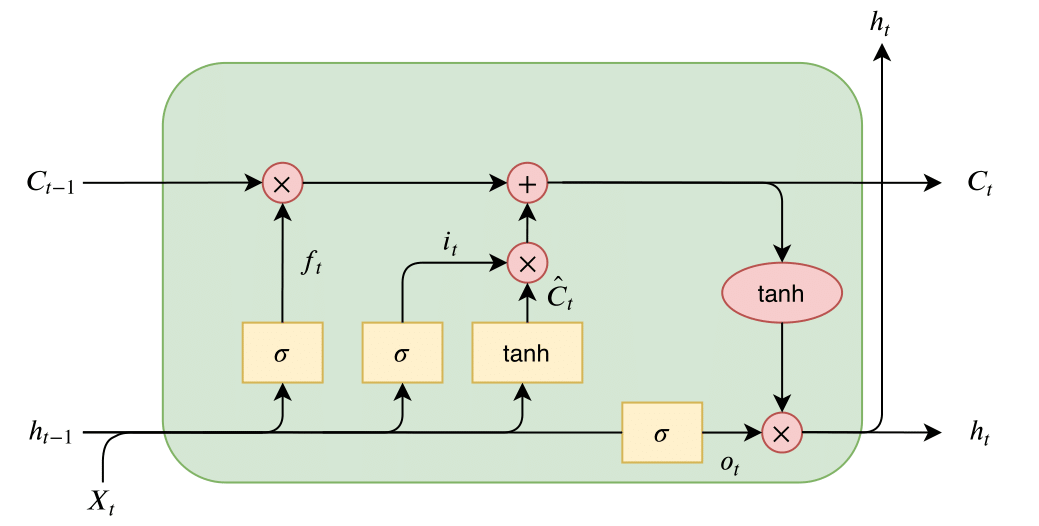
\includegraphics[width=\textwidth]{transformer_images/lstm.png}
		\caption{LSTM}
		\label{fig:LSTM}
	\end{minipage}
	\hfill
	
\end{figure}


\subsection{دروازه‌ها}
دروازه‌ها نقش فیلترهای اطلاعاتی را دارند که جریان اطلاعات را در طول فرایند یادگیری کنترل می‌کنند.

\begin{itemize}
	\item \textbf{دروازهٔ فراموشی \footnote{\lr{Forget Gate}}}
	تعیین می‌کند چه اطلاعاتی از وضعیت سلولی باید حذف شود
	\cite{gers1999learning}.
	
	\begin{equation}
		f_t = \sigma \big( W_f \cdot [h_{t-1}, x_t] + b_f \big)
	\end{equation}

در این معادله، \( f_t \) بیانگر میزان فراموشی برای هر مؤلفه از وضعیت سلولی در گام زمانی جاری است. این مقدار با استفاده از تابع فعال‌ساز سیگموید \( \sigma \) محاسبه می‌شود که خروجی آن بین صفر تا یک قرار دارد. هرچه مقدار \( f_t \) به صفر نزدیک‌تر باشد، آن مؤلفه از وضعیت سلولی بیشتر فراموش می‌شود؛ و بالعکس، مقدار نزدیک به یک نشان‌دهندهٔ حفظ کامل آن اطلاعات در حافظه سلولی است.



	\item \textbf{دروازهٔ ورودی \footnote{\lr{Input Gate}}:}
	تعیین می‌کند چه اطلاعات جدیدی باید به وضعیت سلولی اضافه شود:
	\begin{equation}
		i_t = \sigma \big( W_i \cdot [h_{t-1}, x_t] + b_i \big)
	\end{equation}
	
	\begin{equation}
		\tilde{C}_t = \tanh \big( W_C \cdot [h_{t-1}, x_t] + b_C \big)
	\end{equation}

	که در آن \( i_t \) میزان اطلاعات جدید و \( \tilde{C}_t \) مقدار جدید قابل اضافه‌شدن به وضعیت سلولی را نشان می‌دهد.
	
\item \textbf{دروازهٔ خروجی \footnote{\lr{Output Gate}}:}

	تعیین می‌کند چه اطلاعاتی از وضعیت سلولی به خروجی منتقل شود:
	\[
	o_t = \sigma \big( W_o \cdot [h_{t-1}, x_t] + b_o \big),
	\]
	\[
	h_t = o_t \cdot \tanh(C_t).
	\]
\end{itemize}

\subsection{به‌روزرسانی وضعیت سلولی}
وضعیت سلولی \( C_t \) با استفاده از اطلاعات جدید و قدیمی به‌روزرسانی می‌شود:
	\begin{equation}
		C_t = f_t \cdot C_{t-1} + i_t \cdot \tilde{C}_t
	\end{equation}

این ساختار باعث می‌شود اطلاعات قدیمی مهم حفظ و داده‌های غیرضروری حذف شوند.

\subsubsection{ علت پایداری گرادیان در شبکه های حافظه بلند-مدت کوتاه مدت}
\begin{itemize}
	\item \textbf{حذف ضرب‌های مکرر:}
	برخلاف شبکه های بازگشتی که به ضرب‌های مکرر وزن‌ها و گرادیان‌ها وابسته است، شبکه های حافظه بلند-مدت کوتاه مدت با مسیر جداگانهٔ وضعیت سلولی، از کاهش نمایی گرادیان جلوگیری می‌کند
	\cite{hochreiter1998vanishing}.
	
	\item \textbf{استفاده از توابع سیگموید و تانژانت هیپربولیک:}
	توابع سیگموید در دروازه‌ها و تانژانت هیپربولیک در وضعیت سلولی مقادیر را محدود می‌کنند و مانع از انفجار گرادیان می‌شوند\cite{gers1999learning,goodfellow2016deep}.
	
	\item \textbf{مدیریت اطلاعات توسط دروازه‌ها:}
	دروازه‌های فراموشی و ورودی به مدل اجازه می‌دهند تنها اطلاعات مهم حفظ شود و داده‌های غیرضروری حذف شوند.این موضوع از پیچیدگی محاسباتی غیرضروری جلوگیری می‌کند
	\cite{hochreiter1997long}.
\end{itemize}

\begin{table}[h!]
	\centering
	\resizebox{\columnwidth}{!}{%
		\begin{tabular}{|c|c|c|}
			\hline
			\textbf{ویژگی} & \textbf{RNN} & \textbf{LSTM} \\ \hline
			\textbf{مشکل ناپدید شدن گرادیان} & وجود دارد & برطرف شده \\ \hline
			\textbf{توانایی حفظ وابستگی‌های طولانی‌مدت} & محدود به وابستگی کوتاه‌مدت & بسیار خوب \\ \hline
			\textbf{ساختار دروازه‌ها} & ندارد & دارای دروازه‌های فراموشی، ورودی و خروجی \\ \hline
			\textbf{پایداری گرادیان} & ضعیف & پایدار \\ \hline
		\end{tabular}%
	}
	\caption{مقایسه ویژگی‌های RNN و LSTM}
\end{table}



\subsection{مشکلات کلی شبکه های بازگشتی و ظهور مبدل  ها}
شبکه‌های بازگشتی که به آن ها پرداخته شد توانستند بسیاری از مشکلات و محدودیت‌های مدل‌های اولیه را حل کنند؛
اما همچنان با چالش‌ها و محدودیت‌هایی مواجه بودند که در مسائل پیچیده‌تر، مانند ترجمهٔ زبان یا تحلیل داده‌های بلندمدت و حجیم، مشکلات جدی ایجاد می‌کردند
\cite{hochreiter1997long,goodfellow2016deep}.
این مشکلات در نهایت به پیدایش مبدل‌ها \footnote{\lr{Transformers}} منجر شد\cite{vaswani2017attention}.


\subsection{مشکل وابستگی ترتیبی در شبکه های بازگشتی}
شبکه های بازگشتی داده‌ها را به‌صورت ترتیبی پردازش می‌کنند؛ به این معنی که برای پردازش داده‌های گام زمانی \( t \)، باید تمامی داده‌های قبلی (\( t-1 \)) پردازش شده باشند
\cite{rumelhart1986learning,hochreiter1997long}.
این ویژگی مشکلات زیر را ایجاد می‌کند:
\begin{itemize}
	\item \textbf{غیرقابل موازی‌سازی:}  
	به دلیل وابستگی ترتیبی، پردازش داده‌ها به‌صورت موازی ممکن نیست و همین امر باعث افزایش زمان محاسباتی می‌شود. در داده‌های بلند (مانند متن‌های طولانی یا سری‌های زمانی بزرگ)، این مشکل نمود بیشتری دارد.
	
	\item \textbf{کندی آموزش و استنتاج:}  
	پردازش خطی داده‌ها موجب می‌شود زمان آموزش و پیش‌بینی مدل‌ها به‌شدت افزایش یابد، به‌ویژه زمانی که با حجم زیادی از داده مواجه هستیم.
\end{itemize}

\subsubsection{محدودیت در یادگیری وابستگی‌های بسیار طولانی}
با وجود پیشرفت شبکه های حافظه بلند-مدت کوتاه مدت در یادگیری وابستگی‌های بلندمدت نسبت به شبکه های بازگشتی معمولی، این مدل‌ها همچنان در یادگیری وابستگی‌های بسیار بلند، مانند ارتباط بین کلمات در جملات دور از هم یا درک ساختار کلی یک متن، محدودیت دارند
\cite{hochreiter1998vanishing}:
\begin{itemize}
	\item \textbf{مشکل در داده‌های بسیار طولانی:}  
	حتی در شبکه های حافظه بلند-مدت کوتاه مدت  نیز ظرفیت حفظ اطلاعات محدود است و با افزایش طول توالی، دقت مدل افت می‌کند.
	
	\item \textbf{تأثیر تدریجی داده‌های اولیه:}  
	داده‌های ابتدایی توالی ممکن است با گذشت زمان اهمیت خود را از دست بدهند، چراکه گرادیان‌ها به‌تدریج ضعیف‌تر می‌شوند.
\end{itemize}

\subsection{ پیچیدگی محاسباتی و حافظه در شبکه های بلند مدت کوتاه مدت}
شبکه های حافظه بلند-مدت کوتاه مدت به علت ساختار پیچیده‌ای که شامل چندین ماتریس ضرب (برای دروازه‌های فراموشی، ورودی و خروجی) و به‌روزرسانی وضعیت سلول است، به حافظه و محاسبات زیادی نیاز دارند
\cite{goodfellow2016deep}:
\begin{itemize}
	\item \textbf{نیاز به حافظه بیشتر:}  
	برای ذخیرهٔ وضعیت سلولی و گرادیان‌ها، شبکه های حافظه بلند-مدت کوتاه مدت  به حافظهٔ بیشتری نسبت به مدل‌های ساده‌تر احتیاج دارند.
	
	\item \textbf{هزینهٔ محاسباتی بالا:}  
	در داده‌های حجیم، انجام محاسبات سنگین می‌تواند اجرای مدل را بسیار کند سازد.
\end{itemize}

\subsection{مشکل پردازش وابستگی‌های غیرمتوالی}
شبکه های بازگشتی به‌طور طبیعی برای یادگیری وابستگی‌های محلی و متوالی مناسب هستند. اما در مسائلی مانند ترجمهٔ زبان یا تحلیل متون، روابط غیرمحلی و غیرمتوالی نیز اهمیت دارند
\cite{bahdanau2014neural}.
به‌عنوان مثال، در جمله‌ای طولانی ممکن است کلمه‌ای در ابتدای جمله با کلمه‌ای در انتهای جمله ارتباط معنایی داشته باشد. شبکه های بازگشتی برای یادگیری این‌گونه وابستگی‌ها محدودیت دارند.

\subsection{گرادیان‌های ناپایدار و مشکلات بهینه‌سازی}
با وجود بهبودهایی که شبکه حافظه بلندمدت، کوتاهمدت نسبت به شبکه های بازگشتی معمولی در پایداری گرادیان ارائه داد، هنوز هم مشکلاتی در این شبکه ها وجود دارد که شامل موارد زیر است:
\begin{itemize}
	\item \textbf{مسائل گرادیان‌های ناپایدار:}  
	در توالی‌های بسیار بلند، گرادیان‌ها ممکن است همچنان دچار کاهش یا حتی در مواردی انفجار شوند.
	
	\item \textbf{مشکلات بهینه‌سازی:}  
	در مسائلی با ساختار پیچیده، یافتن مینیمم مناسب تابع هزینه برای شبکه های بازگشتی دشوار است.
\end{itemize}


\begin{itemize}
	\item \textbf{نیاز به مدلی با ظرفیت بیشتر و سرعت بالاتر:}  
	برای مسائل پیچیده‌تر، به مدل‌هایی با تعداد پارامتر بالاتر نیاز است؛ اما این شبکه های بازگشتی به‌دلیل محدودیت در حافظه و پردازش، پاسخ‌گوی این نیاز نیستند.
	
\item \textbf{کارایی در داده‌های چندوجهی \footnote{\lr{Multimodal}}:}برای داده‌هایی که ترکیبی از اطلاعات متنی، صوتی و تصویری هستند،شبکه های بازگشتی توانایی لازم جهت پردازش موازی این اطلاعات را ندارند.
\end{itemize}

در مجموع، وابستگی ترتیبی در شبکه های بازگشتی مانعی اساسی برای استفاده از این مدل‌ها در مسائل پیچیده و بزرگ بود که درنهایت به ظهور مبدل ها منتهی شد
\cite{vaswani2017attention}.
مبدل‌ها با طراحی مبتنی بر موازی‌سازی و مکانیزم توجه \footnote{\lr{Attention Mechanism}}، این محدودیت را برطرف کرده و راه‌حلی کارآمدتر برای پردازش داده‌های ترتیبی ارائه دادند.




